\documentclass[../main.tex]{subfiles}
\graphicspath{{\subfix{../figures/}}}

\begin{document}

\chapter{Overview of Transcriptomic Assays}

\section{Gene Expression Regulation}

Across all cells in all organisms genetic information flows from DNA to RNA to proteins, the central dogma of molecular biology.
Transcription from DNA to RNA and translation from RNA to protein are regulated by numerous mechanisms simultaneously to enable cells to respond to their environment.
This chapter is a brief overview of the transcription and post-transcriptional regulatory mechanisms that contribute to the differential expression of mRNA transcripts with emphasis on the mechanisms present in \textit{Saccharomyces} cerevisiae, Figure \ref{fig:mrna-regulation}. 

\begin{figure}[h]

{\centering 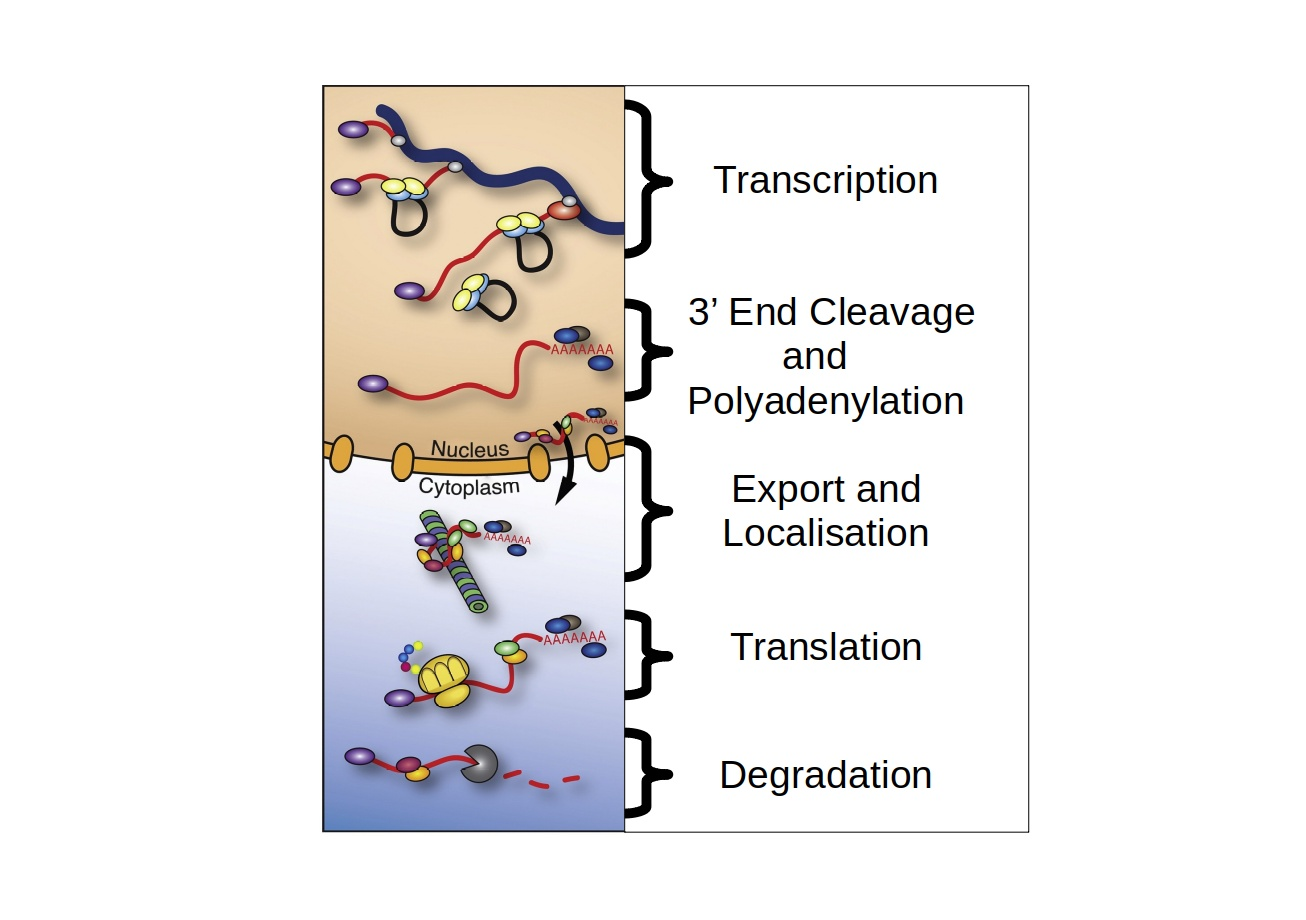
\includegraphics[width=\linewidth]{figures/post-transcriptional-regulation} 

}

\caption[Overview of key mRNA regulatory processes.]{\textbf{Overview of key mRNA regulatory processes.} Several mechanisms act simultaneously to enable cells to respond to their environment through the regulation of mRNA transcripts. Figure adapted from \cite{Corbett2018}}\label{fig:mrna-regulation}
\end{figure}


\subsection{Transcriptional Regulation}

The successful creation of an mRNA transcript from its corresponding DNA template requires the completion of three key transcriptional steps: initiation, elongation and termination.
Initiation of transcription consists of the RNA polymerase II binding to the DNA template upstream of the sequence encoding a protein.
The region where the RNA polymerase II initiates transcription is called the promoter.
In eukaryotes, DNA is wound around nucleosomes and densely packaged in several orders of chromatin structure.
Therefore, the initiation of transcription requires a variety of transcription factors to aid in the unwinding of the chromatin, scanning of regions for promoters, and the binding of RNA polymerase II.
Promoters consist of regulatory sequences that encourage the binding of transcription factors and can be further affected by distal regulatory regions such as enhancers. 

Once transcription is initiated the polymerase begins the sporadic process of elongation from the transcript start site.
For a transcript without introns, the polymerase first transcribes the 5' untranslated region (5'UTR) of an mRNA transcript, then the coding sequence for the corresponding protein, and finally the 3' untranslated region (3'UTR).
However, the process of elongation is highly stochastic with polymerases regularly pausing and even stalling with several accessory proteins required to maintain the process.
Early on in the elongation stage, the 5' end of the pre-mRNA is modified by several enzymes to form a 5'-methyl cap which inhibits degradation and aids translation.
Finally, the termination of transcription remains a relatively unclear process as a distinct termination sequence has not been found.
Instead, the polymerase continues to transcribe the sequence downstream of the 5'UTR.
This downstream terminator region does contain sequences to recruit cleavage and polyadenylation factors.
The still elongating RNA transcript is cleaved at the end of the 5'UTR as dictated by these sequences.
The freely floating pre-mRNA transcript is then bound by a poly(A) polymerase that adds a tail of hundreds of adenine bases to the end of the transcript.
The remaining string of RNA bound to the polymerase and DNA template is degraded by a 5' to 3' exonuclease, which is thought to dislodge the polymerase and terminate transcription \parencite{Alberts2017}.
The terminator can contain multiple cleavage sites leading to transcript isoforms with different poly(A) positions.
Further isoforms can be created as the promoter can contain different transcription start sites leading to transcript isoforms with different exons and 5'UTRs.

\subsection{Post-transcriptional Regulation}

In between the transcription of a nascent RNA transcript and its translation into a sequence of amino acids, a variety of regulatory mechanisms act to remove introns, check for quality control and transport transcripts around the cell.
Some genes consist of regions, called introns, that are between the transcription start and end sites but are not in the final mature transcripts.
Concurrently with or immediately after transcription a group of co-functional RNA and proteins called the spliceosome remove intron segments within nascent RNA transcripts.
The regions that forms the mature mRNA transcript are called exons and a single transcript may consist of 10's of exons spliced together.
Alternative splicing of introns and exons can theoretically produce thousands of different versions of a protein in some Drosophila genes.

Selective degradation of low quality mRNA or transcripts that that are no longer needed is a crucial post-transcriptional regulation mechanism.
The importance of degradation in gene regulation is reflected in the number of redundant processes to degrade transcripts, but the majority of degradation is facilitated by the deadenylation-dependent mRNA decay pathway.
This pathway starts by flagging transcript for degradation by shortening  the poly(A) tail.
Then either the 5'methyl cap is removed to enable 5'->3' degradation by the XRN1 exoribonuclease or 3'->5' degradation is initiated by the exosome attaching to the exposed 3' end. 
A variety of surveillance methods can trigger transcript degradation, including: non-sense mediated decay which checks for premature stop codons, non-stop mediated decay which checks for missing stop codons, and no-go mediated decay which checks for stalled ribosomes on mRNA.
In response to stress or other cause of high load on the degradation machinery, P bodies can form in the cytoplasm that are believed to facilitate degradation as they often contain deadenylation, decapping and degradation factors \parencite{Garneau2007}.

Post-transcription regulation is also known to facilitate temporal and spatial regulation in cells.  
Temporal regulation is common in developmental processes where the order of production of specific proteins is highly regulated. 
For example, in C. elegans lin-4 is a non-coding RNA gene crucial for regulating cell fates during the early stages of larval development \parencite{Wightman1993}. 
Lin-4 is a small RNA that binds to its target mRNA lin-14 and inhibits the translation of lin-14 \parencite{Lee1993}.
Since lin-4 is only expressed at the end of the first larval development stage, lin-14 only is only translationally inhibited late into stage 1, initiating the start of stage 2 \parencite{Olsen1999}. 
Similarly, to establish meiotic chromosome segregation in budding yeast, mRNA encoding cyclin CLB3 is transcribed in stage I of meiosis, but is translationally repressed until stage II of meiosis. 
CLB3 is translationally repressed by the RNA-binding protein Rim4. 
During the transition to meiosis II, Rim4 is phosphorylated which inhibits binding to CLB3 and enables CLB3 to be translated \parencite{Berchowitz2013}. 
Therefore, post-transcription control of CLB3 by Rim4 and of lin-4 by lin-14 depends on the timing of promoter-specified transcriptional control.

Spatial regulation enables centrally transcribed mRNA transcripts to be regulated differently depending on target location of their encoded protein.
In yeast, the Ash1 protein represses mating-type switching only in daughter
cells \parencite{Sil1996}, due to localisation of the ASH1 transcript at the bud tip and subsequent localised translation \parencite{Niednery2014}. 
It is thought that co-transcriptional recruitment of She2 to the ASH1 transcript in the nucleus enables the later recruitment of cytoplasmic factors Khd1/Hek2 and Puf6, factors known for translational repression. 
Furthermore, successful transport of ASH1 to the bud tip by She2-She3-Myo4 complexes depends on translational repression by Khd1 and Puf6. 
Later, phosphorylation of Khd1 and Puf6 by bud-membrane-localised kinases leads to localised translational activation of the ASH1 mRNP \parencite{Paquin2007, Deng2008}.

Another example where the effect of a CRE on a transcript depends on co-localisation with a regulatory kinase comes from the fungal RNA-binding protein Ssd1. 
Yeast cell wall proteins such as Sun4 and Tos6 are translationally repressed by Ssd1 \parencite{Jansen2009}.
It is thought that these transcripts are translationally activated at bud sites after the phosphorylation of Ssd1 by a localised kinase, Cbk1 \parencite{Jansen2009}. 
There is no evidence that Ssd1 directly acts to transport RNA, so this localised activation presumably depends on localisation the recruitment of other RNA-binding proteins to those transcripts \parencite{Hogan2008, Bayne2021}, that then in turn recruit transport machinery.
\newpage


\section{High-Throughput RNA Assays}

\subsection{qPCR}

Polymerase chain reaction (PCR) is regarded as one of the most significant methods in molecular biology.
The accuracy of PCR as a method to produce copies of regions of DNA in a log-linear manner has led researchers to explore its use an accurate method to quantify abundance since its invention in the 1980's \parencite{Saiki1988}.
The quantification of the rate of amplification in real time quickly followed \parencite{Holland1991}, but it wasn't until the 2000's that biochemistry and technology matured into a reliable quantitative PCR (qPCR) method \parencite{Walker2002}.
qPCR is a relatively low-throughput quantification method when compared to the other methods described here.
However, developments in microfluidics and multiplexing target probes are overcoming the bottlenecks in conducting high-throughput qPCR \parencite{Dreier2022}.

The basic principle of PCR consists of the duplication of a region of DNA that is specified by two short nucleotide sequences, called primers, that are designed to be complementary to the start and the end of the region of interest. 
A highly thermotolerant polymerase, adapted from the bacteria \textit{Thermus aquaticus}, is then able to complete the duplication of the region by elongation of the sequence between the two primers \parencite{Saiki1988}.
The duplication cycle is repeated several times leading to an exponential growth in the number of copies of the original region.
The PCR polymerase must be thermotolerant as the duplication cycle is rapidly repeated by raising the temperature to melt the newly created complementary stand away from the original strand before dropping the temperature back down to enable the next round of elongation. 
Quantifying the rate of amplification, is done by introducing dyes that only fluoresce when a region has been successfully duplicated. 
The fluorescence of the sample is measured as the PCR cycle is repeated to determine the exponential growth in duplicates.
Quantitative PCR (qPCR) uses the amplification curve to infer the number of transcripts of the target sequence in the original sample \parencite{Holland1991}.

\subsubsection{qPCR Methods: RNA vs DNA}

qPCR is highly optimised for amplifying DNA fragments using the \textit{Thermus aquaticus} polymerase. 
Therefore, to quantify RNA fragments an additional step is required to create complementary DNA (cDNA) from RNA using a reverse transcriptase. 
Unfortunately, this step can be a significant source of variation and has been determined to be the source of most variation between RNA samples \parencite{Stahlberg2004}. 
The variation in cDNA yield between replicates can be influenced by the choice of reverse transcriptase priming method, the original RNA target concentration and the total RNA concentration in the sample. 
In order for a RT-qPCR experiment to be reproducible the reverse transcriptase step must be optimised and clearly described. 

\subsubsection{qPCR Methods: Taqman vs SYBR Green}

\begin{figure}[h]

{\centering 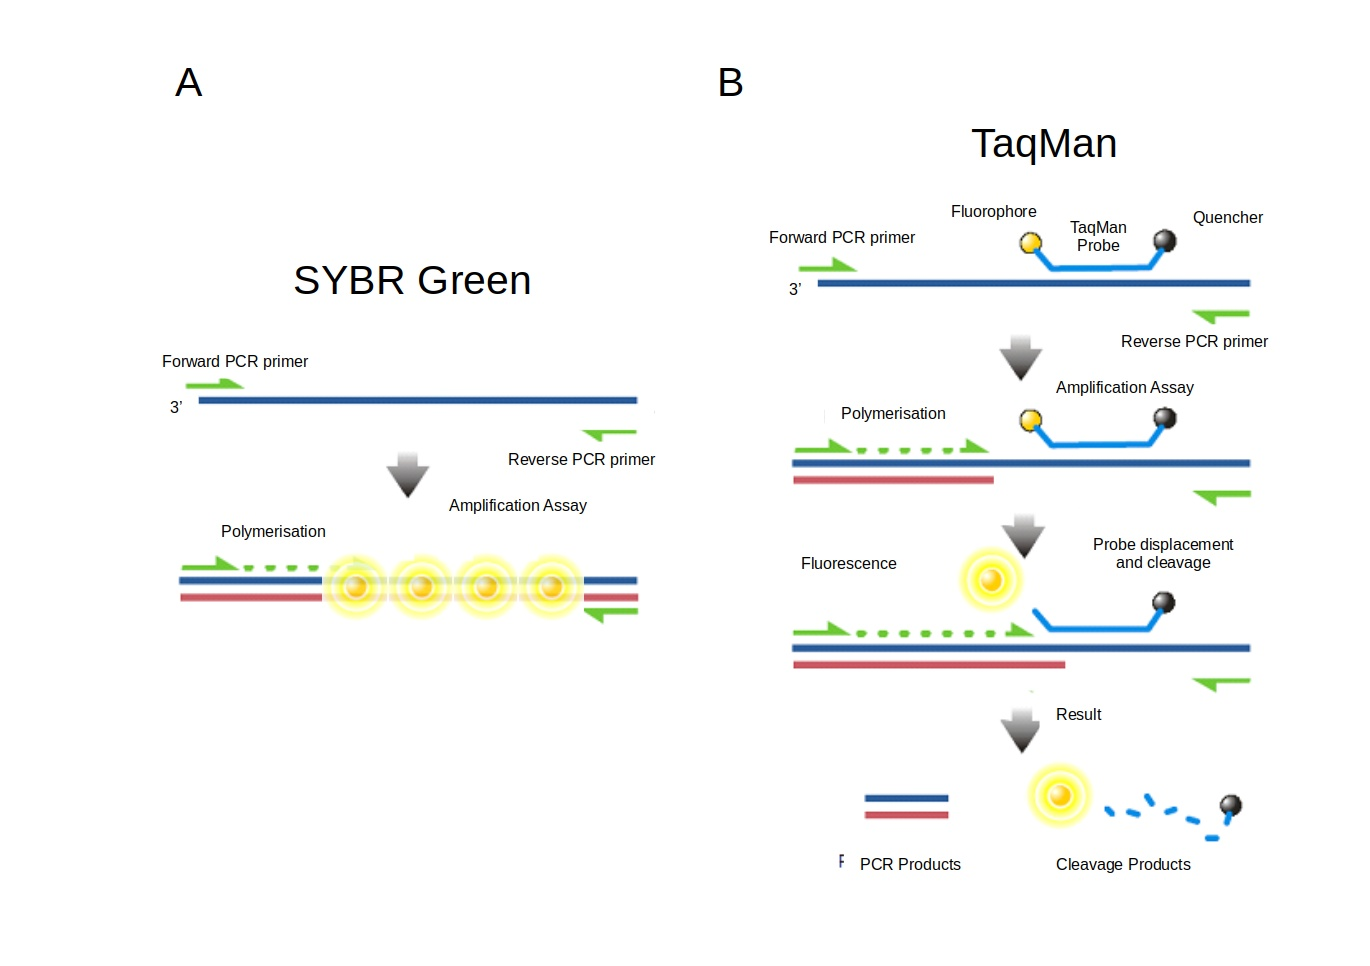
\includegraphics[width=\linewidth]{figures/taqmanvssybrgreen} 

}

\caption[Comparison of qPCR fluorescent probes.]{\textbf{Comparison of qPCR fluorescent probes.} (\textbf{A}) SYBR Green fluorescent probes bind to any double stranded DNA. (\textbf{B}) TaqMan fluorescent probes bind to specific sequences and only fluoresce once detached from their paired quencher post-polymerisation. Figure adapted from Wikimedia Taqman diagram.}\label{fig:qpcr-fluo-tech}
\end{figure}

% https://commons.wikimedia.org/w/index.php?curid=42613619

There are two common types of fluorescent dye used to measure duplicated fragments: TaqMan and SYBR Green.
SYBR Green is a dye that fluoresces when it binds to any double stranded DNA species in the sample, Figure \ref{fig:qpcr-fluo-tech}A.
This leads to it being a cheap and relatively easy to use system, but it is highly susceptible to contamination and it is unable to distinguish between duplicates from different targets. 
TaqMan methods bind the fluorescent dye to a oligonucleotide probe that is designed to attach to the region of interest somewhere in between the two primers. 
The oligonucleotide probe has the fluorescent dye on one end and a quencher on the other.
The quencher stops any excitation emissions from the dye through fluorescence resonance energy transfer. 
However, during elongation, when the polymerase reaches the oligonucleotide probe the probe is hydrolysed separating the dye from the quencher.
Emissions from the fluorescent dye can then be measured and the creation of a new duplicate is detected, \ref{fig:qpcr-fluo-tech}B. 
The introduction of a custom oligonucleotide probe increases the specificity of TaqMan methods and reduces the effects of contamination. 
Also, the abundance of multiple targets can be measured in the same sample by carefully designing different oligonucleotide probes with different fluorescent dyes.
Unfortunately, the design and creation of custom probes causes TaqMan methods to be more expensive and technical. 
The accuracy of TaqMan methods is comparable to the cheaper SYBR Green methods, if correctly conducted \parencite{Tajadini2014}.
Although the limit of detection (LOD) of low copy targets depends on protocol optimisation. 

\subsubsection{Quantifying Abundance: Curve Fitting vs Cycle Threshold}

The exponential limit of the number of duplicates per cycle enables methods that compare abundance across samples. 
Assuming all samples reach the exponential growth stage at the same time then the difference in fluorescence at any cycle of the PCR assay is dependent only on the original copy number. 
However, even if the duplication is perfectly efficient, the amplification curve of duplicates per cycle is not a perfect exponential as there is a limited window through which the number of duplicates will grow exponentially.
The window is defined by limitations in detecting fluorescence at low abundance and the exhaustion of resources at high abundance.
The original copy number can be inferred from the fluorescence if you set a particular fluorescence threshold during the exponential phase and compare the number of cycles needed for a sample to reach it.
Unfortunately, this method assumes both that each sample reaches the exponential phase at the same time and that each cycle doubles the number of duplicates perfectly for each sample. 
An alternative method fits an sigmodal curve to the amplification curve and uses this model to deduce the cycles required to reach a the threshold.
The additional fitting can account for difference in the times to reach the exponential growth phase between samples and can directly account for deviations in perfect duplication \parencite{Swillens2008}. 

\subsubsection{Quantifying Abundance: Relative vs Absolute}

Multiple methods exist for converting cycle threshold measurements, Cq, into quantitative values for sample abundance whilst accounting for experimental and technical noise.
First, qPCR experiments can be designed to measure the relative change in abundance across samples.
Relative abundance measurements depend on the determination of genes that have constant expression across all samples/conditions.
Any change in the gene(s) of interest across samples can then be detected by comparing $\Delta$Cq or the expressions relative to the set of constantly expressed genes.
Normalising the fluorescence to genes with constant expression minimises batch effects introduced by sample preparation, reverse transcription and reactants.
Alternatively, the absolute number of copies of a target in a sample can be estimated.
Absolute quantification of a target requires a preliminary experiment where known initial quantities of the gene of interest are measured with qPCR.
Several amplification curves for the gene of interest, with gradually increasing copies of the gene of interest, are measured to create a collection of standard curves.
Next, the sample from the primary experiment is measured with qPCR and its amplification curve is compared to the standard curves.
The absolute copy number of the gene of interest in the experimental sample can be interpolated.

\subsection{Microarrays}

Microarrays facilitated the creation of the some of the first high-dimensional data sets in transcriptomics.
In the 1980's an assay was published to simultaneously determine multiple specific cell surface antigens through the use of matrix of antibodies fixed to a glass slide \parencite{TseWen1983}.
The opportunity to quantify multiple characteristics of a sample using the same chip led other labs to explore attaching oligonucleotides to a slide, inventing microarrays \parencite{Schena1995}.
The technology enabled the abundance in thousands of genes to be measured simultaneously unlocking studies of gene expression regulation across conditions \parencite{Gasch2000}. 
The assay also benefited from the high quality sequencing of the genomes of multiple species as oligonucleotide probes could be designed to investigate genome-wide behaviours \parencite{Lander2001}.

Microarrays consist of a glass or silicon substrate with spots of DNA printed on in a regular grid. 
Each DNA spot is a complement to a different target which fluoresces when bound with the target. 
In assays to determine differential expression, two colour microarrays are used where each spot contains two fluorescent probes; one to detect the target abundance in the sample of interest and one to detect target abundance in a control or another sample of interest.
A camera detects the level of fluorescence across each spot after excitation by a laser which is used to determine the abundance of that target.  
The two colour microarray assay measures the fluorescence of the two fluorophores and uses the ratio to determine changes in expression.
As the DNA probes have to be designed and printed onto the glass plate their complementary targets have to be decided before conducting the experiment which reduces the opportunity to discover novel regulatory elements \parencite{Schena1995}.

The creation of the high-dimensional data sets with transcript abundance of thousands of genes over dozens of conditions exposed biologists to the n $<<$ p problem.
The size of the data sets acquired were large, but the small number of data points, n, compared to the number of genes and conditions, p, led to low statistical power.
Overcoming the n $<<$ p problem has been a fruitful task for applied statistics with robust methods for sharing expression behaviour across gene and conditions \parencite{Gui2005}.
In addition, the packaging of these novel methods for shrinking variance, calculating penalised t statistics and implementing false discovery rate adjustments promoted the development of quality research software \parencite{Smyth2005, Ritchie2015}.
Distributing the analysis software for microarray arrays led to the open source bioinformatics software repository Bioconductor which has grown to include over 1000 packages for tackling analysis problems across biology \parencite{Huber2015}.


\subsection{RNA-seq}

For 30 years the primary method for sequencing DNA was Sanger sequencing with its massively successful application in decoding the human genome \parencite{Lander2001}. 
The method consists of introducing a di-deoxynucleotide triphosphate (ddNTP) version of one of the four nucleic acids which induces premature termination of elongation when the polymerase incorporates it into a DNA chain.
Due to the stochasicity of elongation the introduction of ddNTP will occur at different stages of duplication leading to the creation of a population of different lengths of copies of a target.
Separating the population by weight using electrophoresis creates bands where the chosen nucleic acid has been replaced by a ddNTP version.
Repeating the process for all nucleic acids enabled a target sequence to be read off \parencite{Sanger1977}.
Similar to qPCR, Sanger sequencing can also be extended to RNA sequencing by introducing a reverse transcriptase step to make cDNA.
The accuracy of the Sanger method means it is remains in use today, but the cost and difficulty of scaling up the method has limited it use.
Instead, the success of the microarray, and its densely packed array of oligonucleotide targets fixed to a solid surface, ushered in a new sequencing technology.

\begin{figure}[h]

{\centering 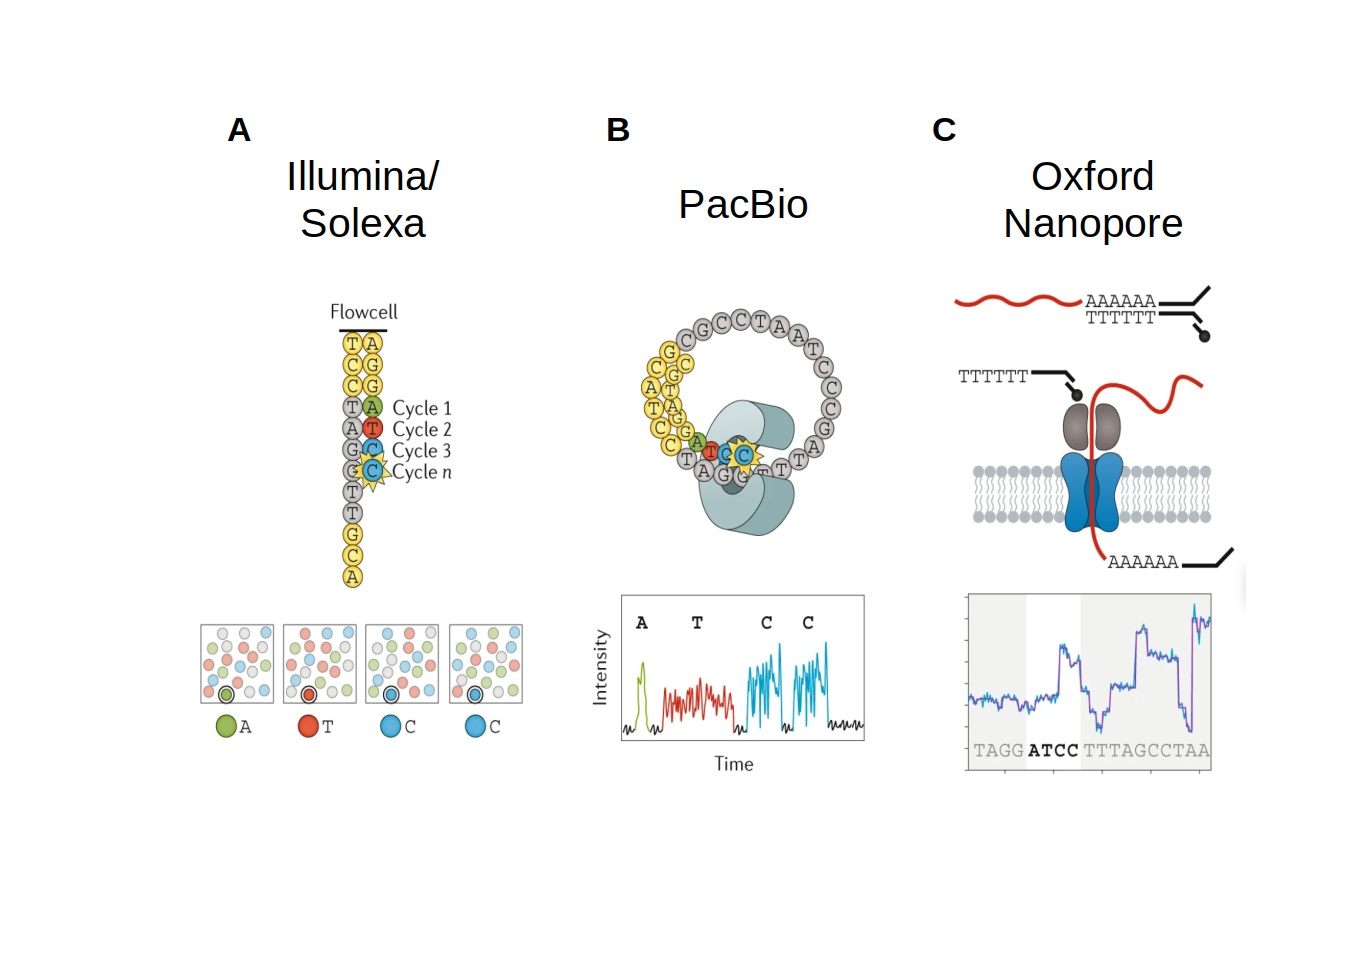
\includegraphics[width=\linewidth]{comparisonofsequencers} 

}

\caption[Comparison of RNA-seq technologies.]{\textbf{Comparison of RNA-seq technologies.} (\textbf{A}) Illumina sequencers attach short fragments to a solid surface called a flowcell. Fluorescent nucleotides create a clear fluorescent spot that identifies the last nucleotide to be attached. (\textbf{B}) PacBio sequencers enable long reads by opening up double stranded DNA into a circle. A polymerase can loop round the circle attaching fluorescent nucleotides that identify the next nucleotide in the sequence. (\textbf{C}) Oxford Nanopore sequencers force nucleotide fragments through protein pores in a membrane. The transmembrane proteins change the current passing through them in response to the nucleotide sequence. The changing in the current can be used to determine the nucleotide sequence. Figure adapted from \cite{Stark2019}}\label{fig:rna-seq-tech}
\end{figure}

\subsubsection{Shotgun Sequencing}

In the early 2000's, several companies competed to overcome the microarray's deficiency in requiring DNA targets to be defined before the experiment \parencite{Rusk2007}.
Solexa (now Illumina) developed adapters that could be ligated to any sample of DNA and facilitate the attachment of the DNA sample to a solid surface. 
Fluorescent nucleotides were created that could terminate elongation in a reversible way.
These nucleotides enabled a base-pair by base-pair cycle of elongation with the identity of the last bound nucleotide being identified by its colour.
Fixing the fragments of DNA to the surface meant islands of duplicates of the original fragment would be created and a clear fluorescent spot could be detected, Figure \ref{fig:rna-seq-tech}A.
Unfortunately, this technology only allowed accurate determination of reads with length <50 nucleotides originally.
As this length is significantly shorter than the majority of sequences of biological interest, the preparation of samples for Solexa sequencing includes a step to break samples in to small fragments, coining the term shotgun sequencing.
The size of the fragments are of the order of 100 nucleotides, which is still larger than the length of reads received from the sequencing machine.
An extension to the single read per fragment method enabled paired reads, one at either end of the fragment, to be detected.
Receiving two reads per fragment improved the accuracy of determining where on the genome a fragment maps to and opened the door to exploring structural variants where fragments were copies of non-adjacent segments of the genome \parencite{Risca2015}.

\subsubsection{Long read Sequencing}

Shotgun sequencing propelled molecular biology into an age of affordable, high-throughput sequencing data.
However, the limit in read size from shotgun sequencing made tasks such as de novo genome assembly and the detection of structural variants significantly difficult.
Long read sequencing technology has now matured with Oxford Nanopore and PacBio offering solutions to read 1000's of nucleotides at a time. 
PacBio sequencers uses fluorescent nucleotides to determine sequences similar to a Illumina sequencer, but instead of binding fragments to a solid surface they form single stranded circles from long segments of double stranded DNA (ddDNA).
Hairpin-shaped SMRTbell adapters are attached to either end of a ddDNA segment creating a closed loop that is opened up into a circle, Figure \ref{fig:rna-seq-tech}B. 
A polymerase is attached to the adapters which can loop round the circle producing multiple copies of both strands of the original ddDNA segment \parencite{Hu2021}.
An Oxford Nanopore sequencer consists of a membrane with 100's of transmembrane proteins that alter their electric resistance when deformed by nucleotides moving through them.  
A current passing through the transmembrane protein then produces a signal in response to the nucleotides moving through the protein, Figure \ref{fig:rna-seq-tech}C.
Machine learning algorithm have been trained to convert the signals in the current into the sequences nucleotides \parencite{Jain2016}.

\subsubsection{Overview of RNA-Seq Based Assays}

As high-throughput RNA-Seq technology has matured, assays to explore a variety of different transcriptome effects have been developed.
With around 80\% of the RNA in a cell being ribosomal, methods to investigate other RNA populations have been developed using enrichment, through poly(A) tail selection, or ribosomal RNA depletion \parencite{Stark2019}. 
Methods that require samples to be PCR amplified before sequencing can add unique molecular identifiers (UMI) to their transcripts to check for biases in duplication \parencite{Kivioja2011}.
Multiplexing methods now allow samples to be pooled together by introducing sample unique barcodes to read adapters which enables ultra-high-throughput methods with one library preparation stage \parencite{Craig2008}.
RNA-protein interactions can be discovered by UV cross-linking transcripts to proteins, pulling out the protein of interest, degrade the protein and analyse the remaining RNA \parencite{Granneman2009}.
Pulse labelling methods can uncover genome-wide transcript production and degradation by introducing a labelled nucleotide and measuring changes in the population of transcripts with that nucleotide \parencite{Chan2018}.
Transcript isomers created by alternative polyadenylation are uncovered by using adapters that ensure reads are anchored to the poly(A) tail \parencite{Pelechano2013}. 
Localisation of transcripts to organelles or membranes can be detected by ultra-centrifugating cell lysate and sequencing the pellet \parencite{Iserman2020}.
Finally, single-cell RNA-Seq technologies are unlocking new cell types and new sources of heterogeneity between homogeneous samples \parencite{Jovic2022}.

\subsubsection{Biases in RNA-Seq assays}

The ubiquitous use of RNA-Seq assays across biology has led to multiple advances in its accuracy and reliability, but many well documented biases remain.
The fragmentation step of RNA-Seq methods introduces a significant gene length bias as longer genes create more fragments \parencite{Oshlack2009}.
GC content of genes changes the reliability of base-calling and alters read-coverage \parencite{Dohm2008}.
RNA-Seq data sets are also highly susceptible to batch effects with total reads per run changing by orders of magnitude \parencite{Auer2010}.
The choice of RNA extraction and enrichment can lead to significant changes in differential expression detection in the same samples \parencite{Sultan2014}.
Meanwhile, poly(A) anchored reads can initiate elongation from internal stretched of adenine instead of the 3'end tail or switch templates mid-elongation \parencite{Balazs2019}.


\subsubsection{RNA-Seq Analysis}

RNA-Seq analysis consists of three core steps: quality control, alignment and counting. The exact quality control steps can change significantly between types of assay.
For example, enrichment of mRNA transcripts using degradation or poly(A) anchors need to be checked for effectiveness by inspecting ribosomal RNA content or tRNA levels.
Meanwhile in the case of single-cell RNA-Seq checking for cases where two or more cells may have accidentally been combined (as doublets are common in occurrence in many technique) is a vital step that is not required for bulk RNA-seq methods.
However, across all methods it will be required to check for sequence amplification biases, calling quality and whether each lane has successfully detected reads.
Once QC has been completed it is then important to remove any adapters and UMI that may have been introduced during the library preparation as these may complicate alignment to the genome. 
Also, it is common to trim the 3' end of reads as errors in nucleotide callings tend to occur at the end. 
If the assay also includes multiplexed samples these need to detected and separated. 
Once the reads have been trimmed and demultiplexed, then they need to be aligned to the genome in order to be able to determine which gene they map to.
A variety of genome aligners are available depending on organism and computing infrastructure limitations.  
BowTie2 is an accurate aligner but it is not splice aware.
Other aligners like STAR or HISAT2 are much better at aligning reads across splicing junctions. 
It is vital that quality control steps are conducted after the alignment step.
If the vast majority of reads do not align to your organism genome there could be a contaminant present. 
Visualising reads on a genome browsers is also important to check for artifacts, strandedness and poly(A) anchoring if appropraite. 
Once the sequences have been aligned the next step is to remove PCR duplicates if UMIs are present. 
If reads aligned to the exactly the same sequence and they have exactly the same UMI, then they are considered duplicates and can be flatten to just one read. 
Finally, with the deduplicated aligned reads fully processed the user can then count the number of reads to each gene or conduct other downstream analyses such as detecting isoforms \parencite{Conesa2016}.

\subsection{RNA-Seq Analysis Pipelines}

The complexity in analysing high volume RNA-Seq data sets has lead to the development of scaleable, flexible and reproducible analysis pipelines.
Assay dependent quality control steps, from removing adapter sequences to mapping to different genome annotations, are often completed by software packages written in different scripting languages.
Workflow languages, such as Nextflow, are able to integrate the inputs and outputs of software in a domain agnostic manner \parencite{DiTommaso2017}.
A community of bioinformaticians are bringing together standardise modules using Nextflow which can be cherry picked to create the best pipeline for any specific RNA-Seq assay \parencite{Ewels2020}.
Furthermore, as differences in software versions contribute to different outcomes workflow languages are being combined with containers: such as singularity and docker \parencite{DiTommaso2015}.

\newpage

\section{Statistical Methods}

The list of statistical methods described has been curated to cover the methods implemented in this thesis.
A comprehensive overview of methods to explore data in the $p >> n$ regime, where $p$ is the number of feature and $n$ is the number of data points, is beyond the scope of this introduction.
This section draws broadly from several sources: the Elements of Statistical Learning \parencite{Hastie2009}, Bayesian Data Analysis \parencite{Gelman2014} as well as relevant review papers \parencite{Greener2021, Wu2015}.
A more representative view of available statistical methods can be found in the original literature.
The list also reveals a pragmatic approach to the frequentist vs Bayesian debate on statistical inference.
Philosophically, the idea that there is an objective truth to be found for any inference task, which motivated the methods within the frequentist ideology, has been unhelpful at best in the pursuit of scientific knowledge.
The Bayesian method of incorporating prior knowledge into model and exploring uncertainty in your results by sampling from a posterior distribution offers a highly applicable structure for compartmentalising sources of error.
However, the efficiency at which frequentist methods can be applied and the quality of available software implementations using them means they are an useful tools in high-throughput data analysis.
Their use as methods to highlight fruitful avenues for further exploration is distinct from their misuse as arbitrators of truth. 

\subsection{Linear Regression}

Predicting observations from linear combinations of variables, or combinations of transformed variables, is the most studied model in statistics as well as being the starting basis of many non-linear models.
A linear model with input vector $X^T = (x_1, x_2, ..., x_p)$ has the form
$$f(X) = \beta_0 +\sum_j x_j\beta_j$$
where $\beta_j$ are the coefficients of interest to be determined.
Assuming Gaussian noise with constant variance, $\sigma^2$, on the observation, y, 
$$y = f(X) + \epsilon \qquad \epsilon \sim N \big(0,\sigma^2\big) $$
we get the likelihood of getting this observation given the predictor variables from
$$L(\beta,\sigma^2;X,y)=(2\pi\sigma^2)^{-1/2}\ exp\Big( -\frac{1}{2\sigma^2} (y-f(X))^2 \Big).$$
The task of linear regression is to find the values of $\beta$ that maximise the likelihood function $L(\beta,\sigma^2;X,y)$.
In frequentist statistics, the objective is to find the point values of maximum likelihood denoted $\hat\beta$.
The most common method to determine $\hat\beta$ is to minimise the residual sum of least squares (RSS) over N observations,
$$RSS(\beta) = \sum^N(y-f(X))^2.$$
Writing the above in matrix form, with $\mathbf{y}$ being the vector of observations and $\mathbf{X}$ the matrix of predictor values for each observation,
$$RSS(\beta) = (\mathbf{y}-\mathbf{X}\beta)^T(\mathbf{y}-\mathbf{X}\beta),$$
differentiating with respect to $\beta$ and setting to zero gives the $\hat\beta$ that minises the RRS
$$\hat\beta = (\mathbf{X}^T\mathbf{X})^{-1}\mathbf{X}^T\mathbf{y}$$
It can be proved that the $\hat\beta$ that minimise the RSS maximises $L(\beta,\sigma^2;X,y)$ as defined above, \parencite{Hastie2009}.

\subsection{Penalised Linear Regression}

In standard linear regression the introduction of more predicting variables will always increase accuracy on a training set as the model begins learning patterns in the noise.
As biological data sets often contain multiple possible predictors and are based on stochastic processes that are inherently noisy a model needs to select biologically relevant predictors.
Penalised linear regression enables variable selection by introducing additional terms to the likelihood that penalise the inclusion of predictors.
The penalty acts on the coefficients of all predictors creating penalised coefficients, $\hat{\beta}$, with general definition

$$ \hat{\beta} =\mathit{argmin}_{\beta} \{L(\beta;x,y) + \mathit{pen}_\lambda(\beta)\}. $$

The penalty function $\mathit{pen}_\lambda(\beta)$ has a parameter $\lambda$ that can be optimised to increase the penalty of adding coefficients and reduce the complexity of the model.
A common penalty function is the $L_n$ norm acting on the magnitudes of the coefficients
$$\mathit{pen}_\lambda(\beta) = \lambda \sum_j |\beta_j|^n.$$
The $L_1$ and $L_2$ norms are regularly implemented with the corresponding penalised regression methods called lasso and ridge regression \parencite{Tibshirani1996, Hoerl1970}. 
The choice of norm does have a significant effect on the regression with the $L_1$ norm able to set penalised coefficients exactly to zero, but the $L_2$ norm is able to deal with collinearity in a more intuitive way by pulling the coefficients of collinear terms to the same value rather than arbitrarily setting some to zero.
Furthermore, work to create a compromise between the two norms has created the elastic-net penalty 
$$\lambda \sum_j (\alpha |\beta_j|^2 + (1-\alpha)|\beta_j|)$$
where $\alpha$ is an additional parameter to be optimised \parencite{Zou2005}. 
This version attempts to combine with variable selection properties of the $L_1$ norm with the collinearity properties of the $L_2$ norm.

\subsection{Bayesian Hierarchical Models}
The Bayesian view of probability is that it represents a reasonable expectation of an event given what we know \parencite{Cox1946}.
The fundamental basis of a Bayesian model is Bayes' Theorem 
$$P(\theta|D) = \frac{P(D|\theta)P(\theta)}{P(D)},$$
which states that the probability of getting certain parameter values given the data, $P(\theta|D)$, is equal to the likelihood of getting this data given the parameters, $P(D|\theta)$, multiplied by the probability distribution over all possible values of the parameter, $P(\theta)$,  divided by the probability of all possible data points, $P(D)$.
$P(\theta|D)$ is known as the posterior distribution, $P(\theta)$ is the prior distribution and $P(D|\theta)$ is the likelihood function.
The theorem was published by Reverend Thomas Bayes in 1763, but the majority of the modern interpretation of Bayesian statistics was developed independently by Pierre-Simon Laplace from 1774 onwards.

Bayesian hierarchical models are designed if the prior distribution itself contains parameters, $\phi$, 
$$P(\theta, \phi|D) = \frac{P(D|\theta,\phi)P(\theta|\phi)P(\phi)}{P(D)}.$$
The higher tiered priors may act across multiple $\theta$ enabling information to be shared across data points to counter the $p >> n$ problem.
As an example, consider a Bayesian implementation of linear regression.
Instead of finding the optimum value of the coefficients, $\hat{\beta}$, we are interested in the posterior distribution given the training data, $P(\beta|D)$.
We can use the exact same likelihood function, but we need to define a prior distribution on the values of $P(\beta)$.
We can recreate the feature selection properties of lasso regression if we use double-exponential distribution centred on zero for the values of $\beta$.
The data, through the likelihood function, must then shift the probability mass above or below zero to suggest non-zero $\beta$ values.
Alternatively, a hyperparameter can be introduced to the double-exponential distribution to select a bias term other than zero.
The hyperparameter could be trained across all terms in the linear model possibly learning that most $\beta$'s are actually 1.

\subsection{Gaussian Processes}

Gaussian processes are a highly applicable tool for Bayesian inference.
Gaussian processes are an extension of a multi-variate normal distribution to infinite dimensions.
It is a collection of random variables with any finite subset having a joint Gaussian distribution \parencite{Rasmussen2005}.
The collection is indexed by a variable typically representing time as Gaussian processes were originally developed to filter and smooth noise time-series data. 
A Gaussian process is fully defined by a mean function, $m(t)$, and co-variance function, $k(t,t')$, of a real function $f(t)$
$$f(t)\sim GP\big(m(t),k(t,t')\big)$$
$$m(t) = \mathbb{E}[f(t)] \qquad k(t,t') = \mathbb{E}[(f(t) - m(t))(f(t') - m(t'))].$$
Unlike linear regression, Gaussian processes act on function space rather than the weight space of the $\beta$ coefficients. 
This means a Gaussian process is able to approximate practically any function and is far more flexible when fitting data that is non-linear and/or correlated.
The definition of the covariance function can give the Gaussian process a variety of useful properties and defines the prior distribution in the Bayesian paradigm.
The squared exponential is a common covariance function,
$$k(t,t') = exp\big(-\frac{1}{2}|t - t'|^2\big)$$
which is infinite differentiable leading to a very smooth Gaussian process.
Akin to any Bayesian method, test data points, $f(t_{*})$, can be sampled by conditioning the joint Gaussian prior distribution on any given training observations, $f(t)$,
$$f(t_{*})\ |\ t_{*},t,f(t)\ \sim\ N\Big(k(t_{*},t)\ k(t,t)^{-1}\ f(t),\, k(t_{*},t_{*})-k(t_{*},t)\ k(t,t)^{-1}\ k(t,t_{*})\Big)$$.
\subsection{Model Selection}

Rigorous assessment criteria are needed to select the best model between a group with different sets of predictors or with different penalties terms, i.e. $\lambda$.
Ideally, the model with the lowest prediction error for all possible data would be selected.
However, since any data set is a subset of all possible data the prediction error of a model can only be approximated.
K-fold cross-validation is a popular method to approximate the prediction error by splitting the available data into K equal sized groups and calculating the mean prediction error when each of the groups in turn is excluded from the train set and used as the validation set
$$CV(\hat{f})=\frac{1}{K}\sum_iL(y_i,\hat{f}^{-k(i)}(x_i))$$
where $\hat{f}^{-k(i)}(x_i)$ is the model trained without the $i^{th}$ group.
The model with the lowest cross validation error is than selected.

Alternatively, the Akaike information criterion (AIC) and the Bayesian information criterion (BIC) can be used to assess models instead of the approximate prediction error.
$$AIC = -\frac{2}{N}\ log\ L(y,f(x)) + 2\ \frac{d}{N},$$
$$BIC = -2\ log\ L(y,f(x))  + d\ log(N)$$
where is $d$ the degrees of freedom, typically the number of predictors \parencite{Schwarz1978,Akaike1971}.
The AIC is derived from the extension of the maximum likelihood principle over the parameters space to include uncertainty over the dimensionality of the parameters, not just the values of the parameters.
Borrowing from information theory, the distance between the ideal model and a candidate model can be measured with the Kullback–Leibler divergence.
The AIC is the asymptotically unbiased estimate of the discrepancy in the Kullback–Leibler divergence between models of different dimensionality.

In the Bayesian paradigm, if we have the posterior probability of two different models, $Pr(f_a|X,Y)$ and $Pr(f_b|X,Y)$ we can calculate the posterior odds 
$$\frac{Pr(f_a|X,Y)}{Pr(f_b|X,Y)}.$$
Model $f_a$ would be selected if the posterior odds > 1, else $f_b$ is selected. 
However, using Bayes theorem
$$\frac{Pr(f_a|X,Y)}{Pr(f_b|X,Y)} \propto \frac{Pr(X,Y|f_a)}{Pr(X,Y|f_a)}$$
which is known as the Bayes factor.
Under some approximations of normality of $Pr(X,Y|f_a)$ it can be shown that
$$log\ Pr(X,Y|f_a) \approx log\ Pr(X,Y|f_a) - \frac{d}{2}\ log(N)$$
which is $-1/2 \times BIC$. 
Comparing the BIC values of multiple models is approximately equivalent to comparing the posterior odds of the models.
It's important to note that both AIC and BIC contain approximations that do not hold in all cases.
A suitable example of model selection with AIC and BIC is with nested models, i.e. when one model contains a subset of predictors contained in the other model.

\subsection{Multiple Hypothesis Testing}

Testing whether an experimental result is statistically significant given some approximate model of the process creating the data is a mainstay of modern research.
The decision on where to place the boundary on what is or is not significant is ultimately decided by the researchers concern about Type I errors; falsely declaring a result significant when it actually arose from the variation in the data, and Type II errors; falsely declaring a result insignificant when it is in fact unexpected.
As high-throughput experiments enable researchers to test thousands of hypothesis simultaneously the susceptibility to Type I errors increases dramatically as more outliers are expected to be detected.
For example, in a frequentist manner, define a result to be significant if there is less than 5\% chance a result like it, or more extreme than it, occurs given the null hypothesis is true.
If we test 100 results using this method, we would expect 5 results to exceed this threshold even if all the results are insignificant, each being Type I errors.
If we test 10,000 results than 500 Type I errors are expected.
Two common methods to account for the increase in Type I errors when testing multiple hypotheses are the Bonferroni correction and the False Discovery Rate (FDR) \parencite{Bonferroni1936, Hochberg1995}.
The Bonferroni correction scales the threshold, $\alpha$, at which a results is considered significant by the number of tests being conducted, $N$,
$$\alpha_{Bon} = \frac{\alpha}{N}.$$
The correction is known to be conservative leading to more Type II errors and lower statistical power.
The FDR is the ratio of Type I errors, $V$, to total number of results called significant, $S$,
$$FDR = E\Big(\frac{V}{S}\Big).$$ 
The FDR method attempts to keep the FDR constant by changing the threshold of significance given the total number of tests to be conducted and the number of results already tested, j,
$$\alpha_{FDR} = \alpha \frac{j}{N}.$$
The FDR method is implemented by ranking the results according to their p-value and comparing the the p-value to a scaled $\alpha_{FDR}$.

\newpage

\section{Research Software Engineering}

The development of high-throughput, multi-omic experiments across the biological sciences has led to an unprecedented demand on software for research.
In the late 90's less than 20\% of research papers mentioned the use of software in their research. 
In 2021, over 70\% of publications stored on pubmed cited the use of software.
Furthermore, articles accepted in the highest impact journals cited more pieces of software on average.
Software developed specifically to answer research questions has rapidly become a cornerstone of the modern empirical method \parencite{Schindler2022}.
The ubiquitous use of software in modern research leads to difficulty in its definition due to its broad range of users, developers and purposes.
However, here we use the definition given by the Knowledge Exchange \parencite{KL2016}:
 
\begin{quote}
"Research software (as opposed to simply software) is software that is developed within academia and used for the purposes of research: to generate, process and analyse results.
This includes a broad range of software, from highly developed packages with significant user bases to short (tens of lines of code) programs written by researchers for their own use."
\end{quote}

Despite its importance, research software development remains a nascent subdomain of software development. 
The academic position of research software engineer was only coined in the late 2000's \parencite{Prause2010} with the creation of the society of software engineers being founded in 2010. 
Exemplary research groups and institutions now exist with the primary aim of developing software to answer, or facilitate others in answering, research questions (Software Sustainability Institute, Alan Turing Institute, etc). 
However, it still remains a domain primarily occupied by self-taught programmers as an aside from their primary domain of expertise. 
The software itself is regularly developed with specific short term goals during the latter stages of scientific inquiry to provide statistical summaries and deduce significant discoveries. 
Therefore, practitioners are rarely trained in the standard development practices that are used across all other professional software development contexts.

\subsection{Software development practices}

%https://f1000research.com/articles/8-1353#ref-19

\begin{figure}[h]

{\centering 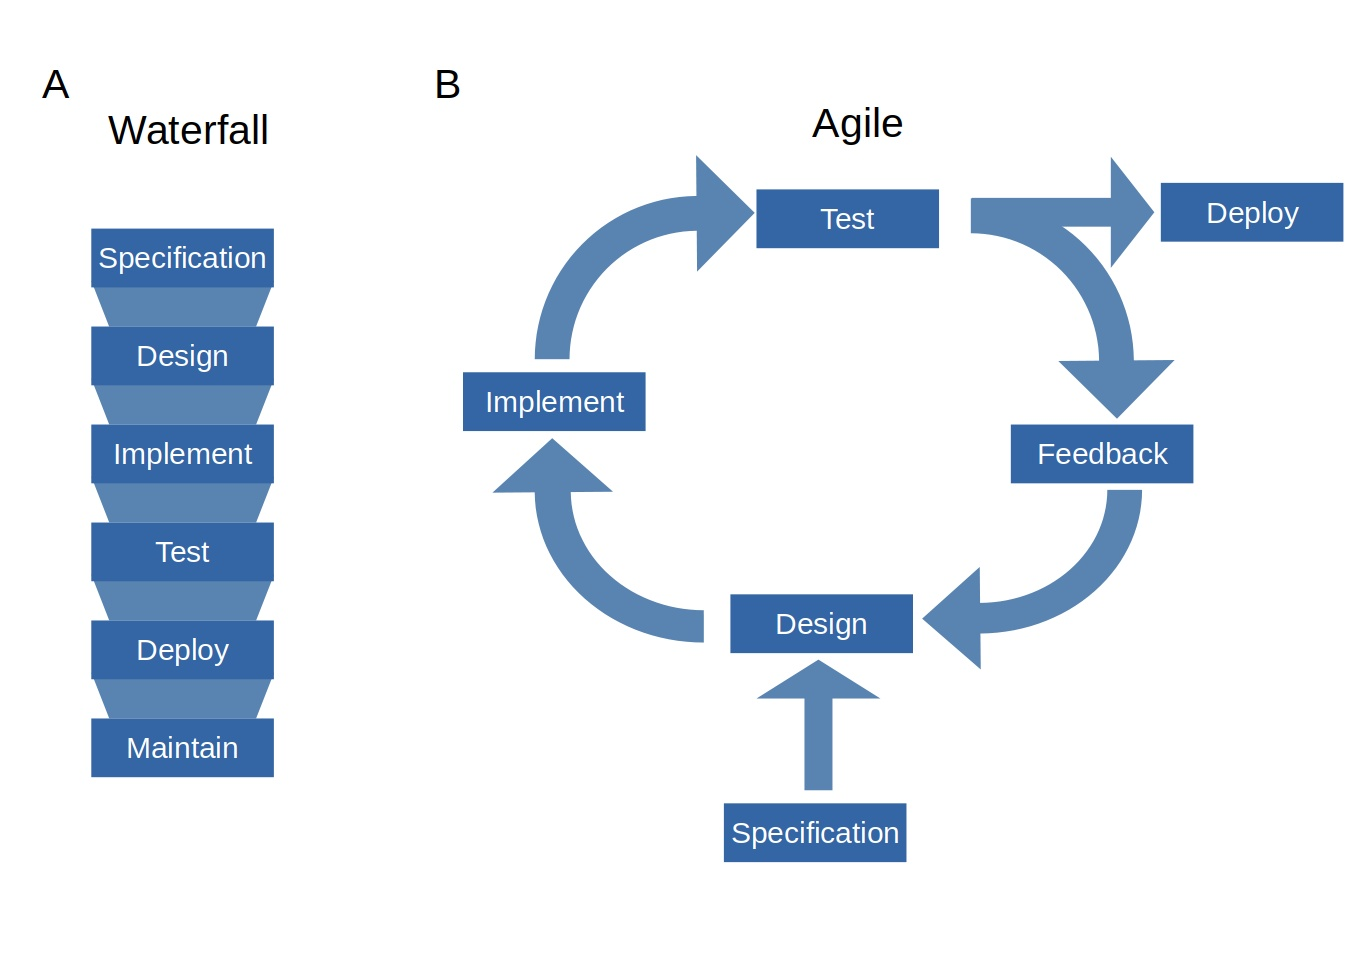
\includegraphics[width=\linewidth]{figures/agileVsWaterfall} 

}

\caption[Comparison of two common software development practices.]{\textbf{Comparison of two common software development practices.} \textbf{A} Waterfall consists of a linear sequence of tasks each of which must be fully completed before moving onto the next. \textbf{B} Agile focuses on gaining feedback as soon as possible by quickly implementing small changes and using feedback to influence the next design stage. }\label{fig:development-practices}
\end{figure}

As software development has become a profession, practitioners have created practices and frameworks to facilitate efficient and rigorous software development.
The practice of don't repeat yourself (DRY) is one of the most commonly implemented to encourage programmers to write short and specific functions to solve regularly occurring tasks. 
Minimising the number of repetitions helps reduce errors (simply from imperfect copying), improves readability and enables faster debugging as compartmentalising tasks into separate functions enables you to test each function separately \parencite{Thomas1999}.
However, DRY does have its opponents as the focus on general abstractions can lead to unreadable code.
For example, a correctly design suite of test is intended to help diagnose bugs during the development stage.
Abstracting error messages to the shortest, most general form can invalid their usefulness in diagnosing bugs.
Therefore, using Descriptive and Meaningful Phrases (DAMP) and repeating how input arguments are defined within each test helps to speed the diagnosis process.

The first software development framework, and the one loosely followed in the sciences, is called waterfall.
Waterfall introduces a structure to the coding practice by outlining a series of stages that are completed linearly, Figure \ref{fig:development-practices}A.
It starts with a detailed specification before moving to development and finally implementation.
Alternative practices generally deviate from the waterfall ethos of leaving implementation to the very last stage.
Instead they prioritise creating a minimal viable product as soon as possible and testing its functionality.
Others even enable the specification to be altered and redefined as the project develops.
The flexibility to redefine the project as it is being developed is why the alternative practices are called agile, Figure \ref{fig:development-practices}B. 

Two common agile practices in industry are scrum and extreme programming.
Scrum is the modern archetypal agile method \parencite{Schwaber2020}.
Instead of fixing the development schedule the project is broken into sprints.
Each sprint iteratively adds some functionality which is reviewed, tested and implemented before moving onto the next.
Constantly reviewing and testing the code enables programmers to catch bugs early and to receive feedback on whether the initial functionality is useful and achievable.
As its name suggests extreme programming pushes the principles of agile programming to the extreme \parencite{Beck2004}.
Updates to the software are tested and implemented on a weekly basis. 
In addition, programmers are expected to conduct paired programming; 
two programmers work together at all times with only one coding while the other verbally dictates what should be added. 
Although this reduces the number of lines of code written per developer, constantly reviewing each others code reduces the number of error which is assumed to negate any reduction in productivity.
Inclusion of agile practices in biomedical research suggests the iterative nature of exploratory research combines effectively with the flexibility of agile software development\parencite{kane2006}.

\subsection{Open source software development}

The software development practices described can be followed with the source code in a private domain, closed source, or in the public domain, open source. 
It is fairly prolific across research to leave any code used in a research paper to be 'available upon request'.
However, the encouragement of open research software practices offers many of the advantages currently seen in industry. 
The success of the Google supported Machine Learning framework TensorFlow showcases the enhanced re-usability, collaboration and accessibility enabled by adopting an open source framework. 

Conducting research software development in an open manner offers several benefits to the developer.
Open source projects have improved findability, accessibility, reproducibility, transparency.
Open science research overall is linked with increased citations, funding bodies placing more weight on open access policies and open project tend to get more coverage in the media \parencite{McKiernan2016}.
A modern parable for open source software development comes for the epidemiological modelling of the spread of COVID-19 by Prof Neil Ferguson at Imperial Collage London.
Crucial to the justification of national lockdowns to kerb the spread of COVID-19, the model was actual developed 13 years prior using undocumented, closed source C++ code.
After six weeks of intense revisions and refactoring, with direct help from Microsoft and GitHub software architects, the model code is now the perfect example of open source research software \url{https://github.com/mrc-ide/covid-sim}.

\subsubsection{Computation and the environment}

A fast growing issue in software development is the contribution of compute to the emission of CO$_2$.
It is estimated that the IT sector will be responsible for 20\% of the world's CO$_2$ production by 2030 \parencite{CCEE2020}. 
Incorporating carbon footprint estimates into coding specifications and benchmarking published code may be the norm in the future \parencite{Lannelongue2021}.
The use of software and the versions of software may increase speed, but at the cost of increased energy requirements.
For example, HISAT2 and STAR are two commonly used sequence aligners noted for significantly different speeds and memory requirements.
Previous research has noted that memory usage is overtaking CPU as the leading energy consumer in servers.
Even just the allocation of memory to a task can significantly increase energy usage with 90\% of energy spent on maintaining memory in the background regardless of load \parencite{Karyakin2017}.
On a broader note, the standard implementations of agile software development could be questioned with weekly or daily testing considered computationally wasteful.



\subsection{GUIs or CLIs}

In the initial stages of developing any piece of software the developer decides how the user will interact with the software: point and click with a graphical user interface (GUI), or programmatically with a command line interface (CLI).
Statistical software has been developed using GUIs since the Macintosh as developers attempted to reduce the mental load of conducting statistical analyses by removing the programming requirement \parencite{ValeroMora2012}. 
The better user experience in a GUI over a CLI \parencite{Staggers2000} is paid for by larger development and maintenance costs.
A GUI also tends to become outdated as there is not an intuitive structure to create and expand a GUI in response to novel statistical methods and problems \parencite{Unwin2012}.
Finally, analyses using CLIs tend to be more scalable and reproducible that GUI analyses as they are difficult to intergrate with modern workflow systems. 


\subsection{Software documentation}

Software development methodologies from Waterfall to Extreme focus entirely on efficient and accurate frameworks for writing code, but none explicitly state time for writing documentation. 
Poor documentation deters user from using you software by extending the its learning curve and increases the likelihood of inappropriate applications of software as users may not understand its assumptions and functionality.
Previous studies have recognised three categories of documentation: documentation of decisions, why did you chose this problem to solve and why did you chose this particular method to solve it; documentation of product, what is contained within this software implementation and how do users interact with it; and documentation of technicalities, how developers created the software and how maintainers can contribute to it. 
Any software intended to be shared contains some product documentation, but few research software projects outline technical details and fewer still mention any decisions made in development \parencite{Geiger2018}.

\subsection{The importance of research software documentation}

The literature on developing useful and usable bioinformatics software is unanimous on the need to document how and why to use a package \parencite{Wilson2017,Taschuk2017,Leprevost2014}.
Furthermore, the widely popular Findable, Accessible, Interoperable and Reusable (FAIR) principles for scientific data have now been extended to research software and documentation is at the forefront: "R1. Software is described with a plurality of accurate and relevant attributes" \parencite{Barker2022}.
Widely used software repositories, such as Bioconductor, demand long-form documentation outlining the decisions made in creating a package as well as how to interact with it in order for the package to be accepted \parencite{Gentleman2004}.
Documentation acts as "a resource for learning and a second role: as an advertisement for the software project" and the current health of a project \parencite{Geiger2018}.
Finally, poor documentation is limiting the scientific research as archived and outdated software packages are still being used because they are well documented.

As well as being best practice for ensuring code usability, quality documentation can also improve the quality of the code itself.
Documentation of technicalities and a suitable code of conduct can help develop a community of maintainers that can fix bugs, update dependencies and add functionality together \parencite{Community2022}.
Open source documentation combats unconscious knowledge as developers of the code can overlook key pieces of information for using the software that can only be rectified by new users contributing to the package \parencite{Hermann2022}.


\subsection{Understanding the rise of poor research software documentation}

The existence of multiple categories of documentation leads to a diverse set of reasons why users may find a software’s documentation insufficient.
Previous research found common issues were based on factually incorrect statements in the documentation, sections of code/functions without any documentation at all or documentation becoming out of date with the latest package versions.
Other issues discuss the difficulty at which API documentation could be found and searched at all, exactly what terms meant in specific contexts and not having quality translations of documentation in other languages.
As expected, a complete lack of documentation is the most common issue but on the other extreme is dense, unintelligible documentation that is difficult to maintain and search \parencite{Aghajani2019}.

Every developer knows the importance of documentation, but new software continues to be created with poor documentation.
In a 2017 GitHub survey of OSS contributors, 93\% reported that “incomplete or outdated documentation is a pervasive problem” but “60\% of contributors say they rarely or never contribute to documentation” \parencite{Geiger2017}.
Software documentation typically is the least credited part of software development with little time or funds allocated to its development.
In industry, documentation writers are first to go in times of economic difficulty \parencite{Forward2002}.
In academia, research posts are only for a few years so there is little time, or motivation, for the developer to respond to user queries \parencite{Hermann2022}.
Simultaneously, writing software documentation requires the most diverse set of skills and experiences to enable people from different backgrounds and knowledge to jump right in at an appropriate level \parencite{Geiger2018}.


\subsection{Improving research software documentation}

The solutions to improving research software documentation target the three main causes: lack of understanding of how to document software, loss of focus on the audience and little reason to allocate time to writing documentation. 
Developers of research software need to be taught the pedagogy of software documentation and the tools available to support documentation.
Institutes such as the Software Sustainability Institute and the Turing Institute are supporting training and learning resources, but little is mentioned in formal data-analysis training. 
Similar to the frameworks developed for software development, documentation frameworks need to be popularised to acknowledge the continued effort required to keep documentation relevant, accurate and searchable.
Diataxis is a popular framework for creating documentation along its two axis of knowledge: theory vs practice and acquisition vs application. 
They separate software documentation into four rough types: Tutorials, practical, and application knowledge; How-tos, practical, and acquisition knowledge; references, theoretical, and acquisition knowledge; and explanations, theoretical, and application knowledge.
Researchers and software developers need to be rewarded for creating usable and documented software packages.
Recognising and correctly citing the use of other peoples software should be as important as citing other people's research papers.
Long-lasting code requires long-term funding which need to be supported by suitable grants judged on appropriate criteria \parencite{Goble2014}.
Funding bodies and journals have acknowledged across the board that research data needs to be FAIR and hopefully the FAIR principles for research software will be equally supported.
% https://www.rd-alliance.org/system/files/FAIR4RS_Principles_v0.3_RDA-RFC.pdf.
 %https://diataxis.fr/
% https://www.proquest.com/docview/304387282
\newpage
\end{document}
